% src/figures/pitch/filters.tex
% Band-Pass Filter Block Diagram
%
% Author: Edward Silva
% Creation Date: 10 November, 2026
% Last Update: 10 November, 2026
%
% Source of Figure 1 on the Pitch tracking page. The signal x[n] goes through a Butterworth
% high-pass filter, then a Butterworth low-pass filter, and comes out as h[n]. Text is set in
% Source Serif 4 with italic text for the symbols, so no math font is loaded. Strokes and text are
% ink #16233a, boxes are white, and lines are 0.6 pt.
%
% Where this file is used within the repository:
% - Builds src/figures/pitch/filters.svg, which src/content/docs/projects/dsp-final.mdx shows
% - npm run figures then writes filters-dark.svg from filters.svg
%
% Usage:
% $ `mkdir -p /tmp/fig && xelatex -no-pdf -output-directory=/tmp/fig src/figures/pitch/filters.tex`
%   : Writes /tmp/fig/filters.xdv
% $ `dvisvgm --no-fonts --exact-bbox -o src/figures/pitch/filters.svg /tmp/fig/filters.xdv`
%   : Writes filters.svg with the glyphs as paths
%
% Copyright (c) 2026 Edward Silva. All rights reserved.

\documentclass[border=1pt,dvisvgm]{standalone}
\usepackage{fontspec}
\usepackage{xcolor}
\usepackage{tikz}
\usetikzlibrary{arrows.meta,positioning}

\setmainfont{Source Serif 4}
\definecolor{ink}{HTML}{16233A}

\newcommand{\sym}[1]{\textit{#1}}
\newcommand{\sub}[1]{\textsubscript{#1}}

\tikzset{
  every node/.style={text=ink},
  block/.style={
    draw=ink, fill=white, line width=0.6pt, rectangle,
    minimum width=7.6em, inner sep=0.5em, align=center, font=\small
  },
  wire/.style={draw=ink, line width=0.6pt, -{Latex[length=5pt,width=4pt]}}
}

\begin{document}
\color{ink}
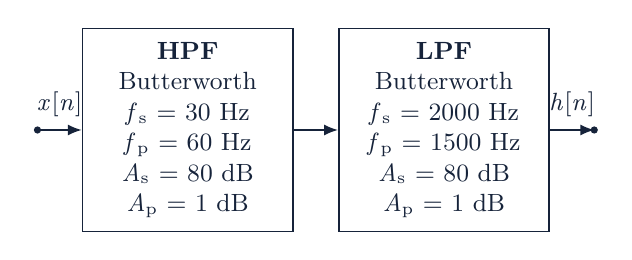
\begin{tikzpicture}[font=\small]
  \node[block] (hpf) {\textbf{HPF}\\Butterworth\\\sym{f}\sub{s} = 30 Hz\\\sym{f}\sub{p} = 60 Hz\\\sym{A}\sub{s} = 80 dB\\\sym{A}\sub{p} = 1 dB};
  \node[block, right=1.6em of hpf] (lpf) {\textbf{LPF}\\Butterworth\\\sym{f}\sub{s} = 2000 Hz\\\sym{f}\sub{p} = 1500 Hz\\\sym{A}\sub{s} = 80 dB\\\sym{A}\sub{p} = 1 dB};
  \draw[wire] ([xshift=-1.6em]hpf.west) -- (hpf.west) node[midway, above=0.1em] {\sym{x}[\sym{n}]};
  \draw[wire] (hpf.east) -- (lpf.west);
  \fill[ink] ([xshift=-1.6em]hpf.west) circle (1.3pt);
  \fill[ink] ([xshift=1.6em]lpf.east) circle (1.3pt);
  \draw[wire] (lpf.east) -- ([xshift=1.6em]lpf.east) node[midway, above=0.1em] {\sym{h}[\sym{n}]};
\end{tikzpicture}
\end{document}
